\chapter{Mathematical Development}
\label{mathchapter}
Some of the contents of this chapter are reprinted, with permission, from \
\begin{enumerate}
\item[\cite{ch4_10_bai2016sum}] Bai, S., \& Skodje, R. T. The Sum Over Histories Representation for Chemical Kinetics: A Quantitative Theory Based on Chemical Pathways. \textit{International Reviews in Physical Chemistry}, 35(4), 539-567. \textbf{2016}
\end{enumerate}
\section{Introduction}
\label{ch2:sec:intro}
The application of the SOHR approach requires a well-defined chemical model, and
thus we begin with a review of conventional kinetics. The chemistry of a reaction network
is traditionally modeled using mass-action kinetics where the concentrations for
$N$-species are solved as functions of time, i.e. $\left(X_1(t), X_2(t), \cdots X_N(t)\right) = X(t)$. We shall
assume that the chemical model under consideration consists of M elementary chemical
reactions in a homogeneous well-stirred reactor
\begin{equation}
\label{ch2:eqn1}
\sum_{i}^{reactants}{{\bar{v}}_{i,j}S_i} = \sum_{i}^{products}{v_{i,j}S_i} ~~~j=1,\cdots,M 
\end{equation}
involving $N$ distinct chemical species $S_i$ which have concentration $X_i$. The molecularities,
$v_{i,j}$ and ${\bar{v}}_{i,j}$, enforce the elemental mass conservation for each reaction indexed by
j. The rate of each reaction is given by a well-defined rate law, $R_j(\mathbf{X})$. (Nothing
prevents the SOHR method from being applied to problems with time-dependent rate
coefficients although we do not explicitly include a t-dependence in the formulae.) The
continuous concentrations of the distinct species $S_i$, $X_i(t) \geq 0$, can be expressed as solutions
of the differential rate eqn. \ref{ch2:eqn1}. The rate equations are given by
\begin{equation}
\label{ch2:eqn2}
\frac{dX_i(t)}{dt} = F_i(\mathbf{X})
\end{equation}
The net rate for species $S_i$, $F_i(\mathbf{X})$, is composed of the source and sink terms from each
elementary reaction in the mechanism, i.e.
\begin{equation}
\label{ch2:eqn3}
F_i(\mathbf{X}) = \sum_{j}^{sources}{v_{i,j}R_j(\mathbf{X})} - \sum_{j}^{sinks}{{\bar{v}}_{i,j}R_j(\mathbf{X})}
\end{equation}
The solution to eqn. \ref{ch2:eqn2} can become difficult if the model grows very large or if
multiple time-scales yields a high degree of stiffness in the equations.
\newline
\paragraph{}
We note briefly that another approach to kinetic modeling exists that is based on
the methods of stochastic modeling. There, a discrete atomistic representation is
adopted in which ensembles of molecules react according to a stochastic model.\cite{ch1_IRPC_33_van1992stochastic}
This viewpoint, pioneered in the early work of McQuarrie\cite{ch1_IRPC_34_mcquarrie1967stochastic} and later by Gillespie
and coworkers\cite{ch1_IRPC_35_gillespie1976general,ch1_IRPC_36_gillespie2013perspective,ch1_IRPC_37_gibson2000efficient}, makes use of MC sampling methods to propagate large ensembles
of discrete molecules. This method has proved useful in problems, such as those
involving biomolecules, where concentrations are very low and hence the fluctuation in
the number of molecules can play a role. A mathematical representation for this technique
involves the chemical master equation (CME), where one solves for the probability
distribution function $P\left( \mathbf{x},t\vert {\mathbf{x}}_0,t_0 \right)$. The variables $\mathbf{x} = (x_1,x_2,\cdots x_N)$ represent the
number of species molecules in a given volume and $P\left( \mathbf{x},t\vert {\mathbf{x}}_0,t_0 \right)$ is the probability that
the species are populated by x at time t given that they were populated as ${\mathbf{x}}_0$ at time $t_0$.
Obviously, the solution to the CME contains vastly more information than does the
mean field eqn. \ref{ch2:eqn2}. It is also much more difficult to solve the CME than the
concentration based kinetics equations. The most effective numerical techniques for
solving the CME involve averaging many stochastic trajectories which simulate the
time evolution of a large ensemble of molecules.
\section{Defining Chemical Pathways}
\label{ch2:def_path}
The basic units of description in the SOHR are the chemical pathway themselves. The
pathways represent the condition of a chemical moiety as it moves from species to species
due to the action of the elementary chemical reactions. Taken collectively, these
pathways describe the entire chemistry of the model. In order to quantitatively apply
the SOHR to practical systems, we require an unambiguous procedure to define and
enumerate these pathways. One can imagine a reaction pathway as either a sequence of reactions or a sequence of species that propagates the chemical moiety through the
chemical network. If the reaction sequence is $R_1$, $R_2$, $\cdots$, $R_n$, then the product molecule
from reaction $R_i$ should be a reagent molecule for the reaction $R_{i+1}$. In terms of species,
on the other hand, there will be a sequence of $n + 1$ moiety-containing molecules $S_0$,
$S_1$, $\cdots$, $S_n$ that are connected by n elementary reactions. For a general non-linear mechanism,
it is necessary to specify both the reactions and the species along the reaction
pathway in order to achieve uniqueness. Indeed, the same reagents may yield different
products or the same products may result from different reagents, depending on which
reaction occurs. For example, if we imagine the gas-phase combustion of the methanol
molecule, CH$_3$OH, a hypothetical three-step chemical pathway is $\textcolor{red}{\textbf{C}}\text{H}_3\text{OH}(+\text{OH}) \xrightarrow[\text{R}_{1}]{\makebox[0.6cm]{}} \textcolor{red}{\textbf{C}}\text{H}_3\text{O} (+\text{O})  \xrightarrow[\text{R}_{2}]{\makebox[0.6cm]{}} \textcolor{red}{\textbf{C}}\text{HO} (+\text{OH}) \xrightarrow[\text{R}_{3}]{\makebox[0.6cm]{}} \textcolor{red}{\textbf{C}}\text{O}$ which yields the CO product. Obviously the reagents in first step of this path, ${\textbf{C}}\text{H}_3\text{OH}+\text{OH} \xrightarrow[\text{R}_{1}]{\makebox[0.6cm]{}} {\textbf{C}}\text{H}_3\text{O} + \text{H}_2\text{O}$, could have equally well yielded the chemically distinct products ${\textbf{C}}\text{H}_2\text{OH} + \text{H}_2\text{O}$, which must be described by a separate
reaction $R_1^{\prime}$. Likewise, the distinct reaction ${\textbf{C}}\text{H}_3\text{OH}+\text{H} \xrightarrow[\text{R}_{1}]{\makebox[0.6cm]{}} {\textbf{C}}\text{H}_3\text{O} + \text{H}_2$ is a different reaction route that connects the followed species CH$_3$OH and CH$_3$O.
\newline
\paragraph{}
In most numerical applications of the SOHR methodology, we adopt a followed-atom
approach for the definition of the chemical pathways. Thus, an atom in a reagent
species is ‘tagged’ at the beginning of the simulation, $t_0$, and it is followed as it hops
between species due to reaction until the final time $t_f$. For example, the carbon atom in
the above pathway has a history $(t_0 \vert S_0R_1S_1R_2S_2R_3S_3|t_f)$ where the C-containing species
are $S_0 = \text{CH}_3\text{OH}$, $S_1 =\text{ CH}_3\text{O}$, $S_2 = \text{CHO}$, and $S_3 = \text{CO}$, and the reactions are
$R_1 = \text{CH}_3\text{OH} + \text{OH} \rightarrow \text{CH}_3\text{O} + \text{H}_2\text{O}$, etc. These histories represent pathways through
species space which deliver the chemical moiety (in this case a C-atom) from the
reagents to the products. A general pathway that delivers a C-atom from CH$_3$OH to CO
may be arbitrarily long and thus may consist of an arbitrarily long sequence of reactions.
The numerical utility of the SOHR method requires that only a finite and manageable
number of the pathways are actually required to converge meaningful results.
\newline
\paragraph{}
From our atomistic viewpoint, the reactions $R_1, R_2 \cdots R_n$ are a sequence of random
events that occur instantaneously at times $t_1, t_2 \cdots, t_n$. Consistent with the time-ordering
along the pathway, the times must satisfy the inequalities $t_f > t_n > t_{n - 1} \cdots > t_1 > t_0$.
Hence, we can further specify the path by noting the reaction times along with the initial
and final times, i.e. $\left(t_0 \vert S_0R_1(t_1)S_1R_2(t_2)S_2R_3(t_3)S_3|t_f\right)$. The chemical histories of an
atom that goes from an initial to a final species may be, in principle, of any length ‘n’
passing through n + 1 species via n reaction steps occurring at times $t_f > t_n > t_{n - 1} \cdots > t_1 > t_0$. In Fig. \ref{ch2:fig1} we show a schematic of several chemical pathways that deliver a
tagged atom from species $S_1$ to species $S_7$. In the upper panel, we show these pathways
on a chemical graph. In the lower panel, we show trajectories that follow these paths
for a particular set of reactions times.
\begin{figure}[htbp]
	\caption[Two representations of chemical histories]{Two representations of chemical histories. In the upper panel, four chemical pathways
followed by a ‘tagged atom’ are displays on a chemical graph. The species are represented as
vertices and reactions are lines (or edges). In the lower panel, four analogous stochastic trajectories
are plotted as species number vs. time. The time-dependence of the trajectory corresponds to
a Markov chain of random reactions.}
    \begin{center}
	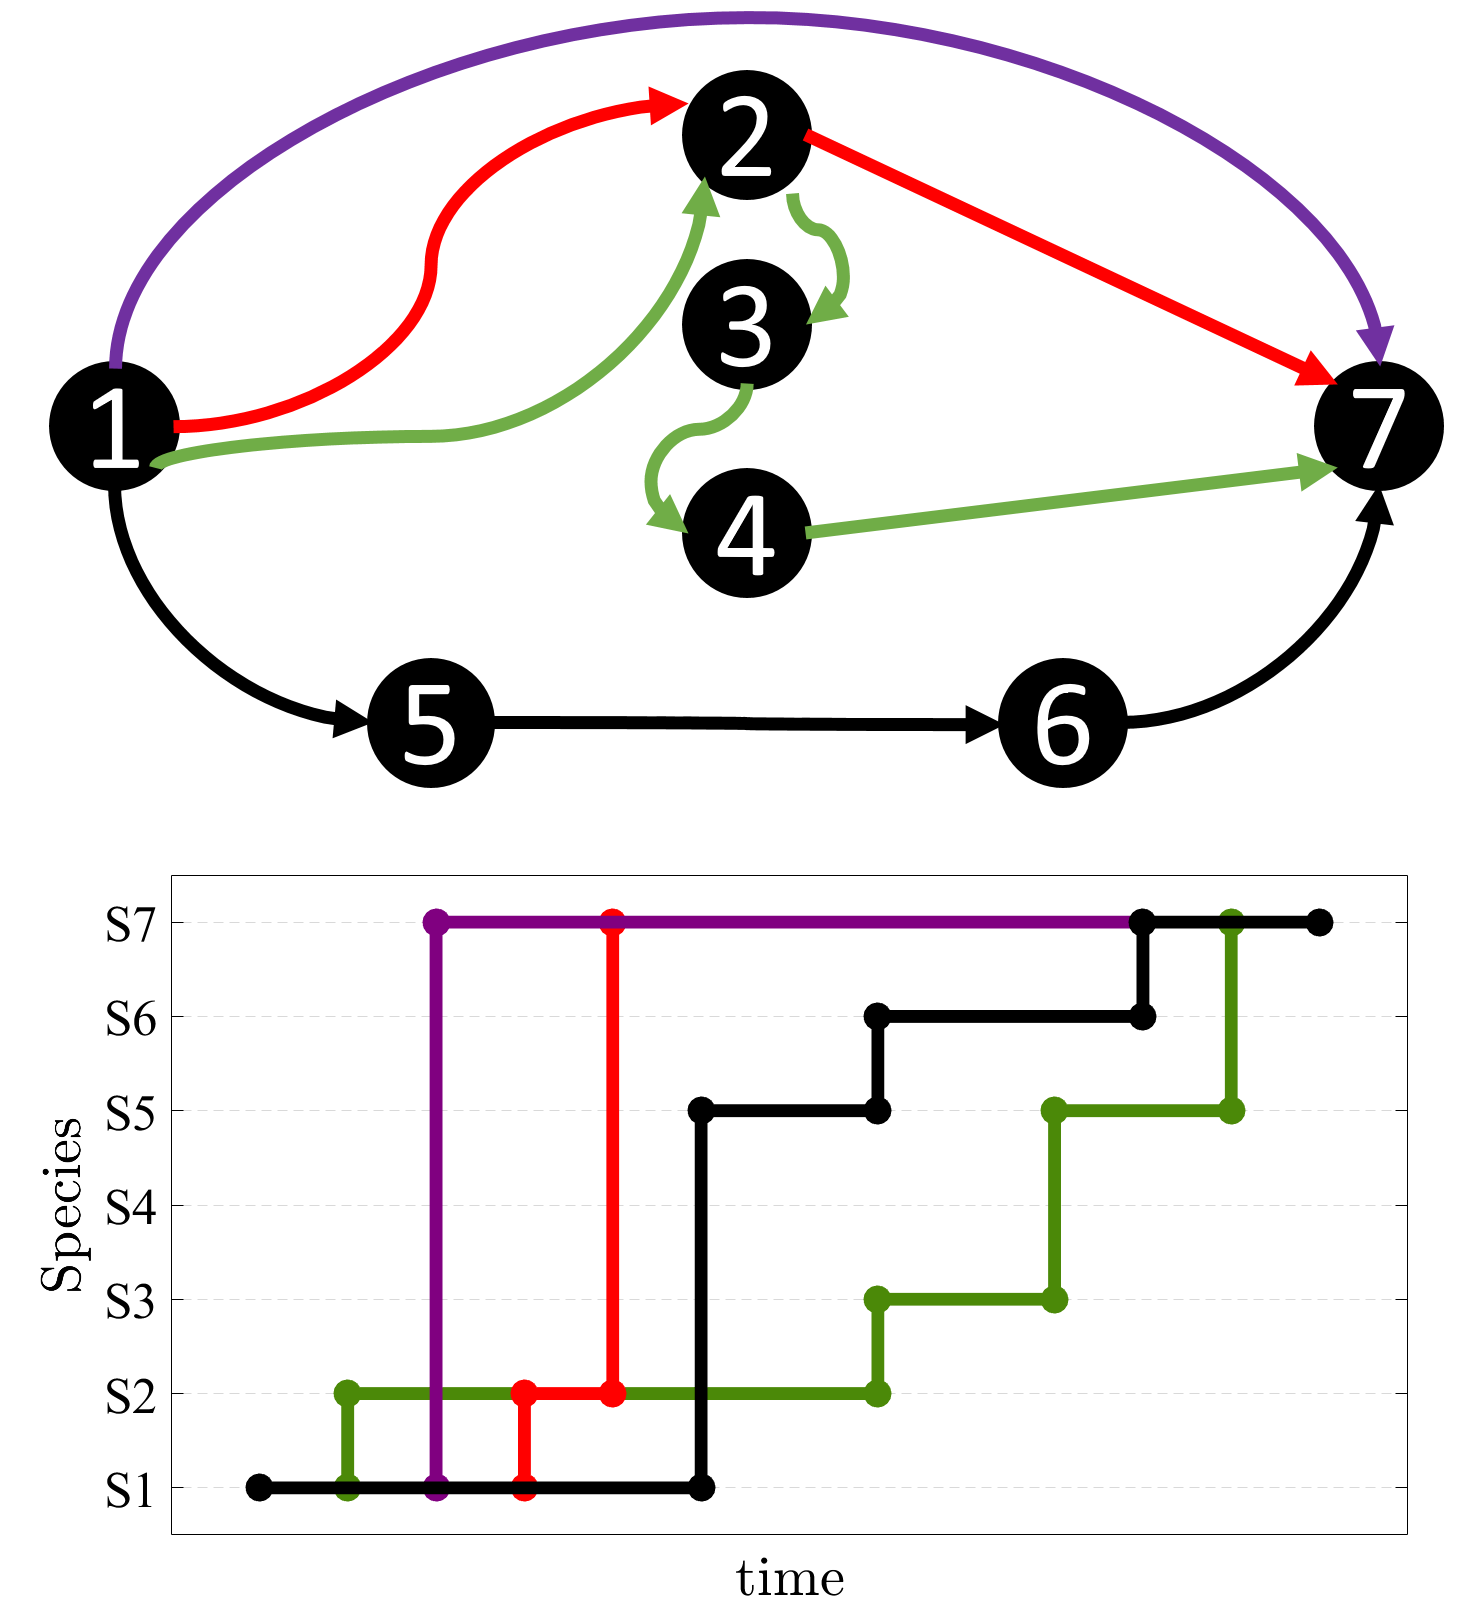
\includegraphics[width=100mm]{figs/chapter2/fig1.png}
    \end{center}
\label{ch2:fig1}
\end{figure}

\section{Pathway Probabilities}
\label{ch2:sec:path_prob}
The essential step that enables the SOHR to be used as a quantitative model of the
reaction kinetics is the assignment of a numerical probability for a given chemical pathway.
We consider a general pathway consisting of n-reactions and n + 1-species, 
i.e. ${\textbf{S}}_{0} \xrightarrow[\text{R}_{1}]{\makebox[0.6cm]{$t_1$}} {\textbf{S}}_{1}  \xrightarrow[\text{R}_{2}]{\makebox[0.6cm]{$t_2$}} {\textbf{S}}_{2} \cdots {\textbf{S}}_{n-1} \xrightarrow[\text{R}_{n}]{\makebox[0.6cm]{$t_{n}$}} {\textbf{S}}_{n}$ where the followed-atom hops from S$_i$ to S$_{i+1}$ at time t$_{i+1}$ due to elementary reaction R$_{i+1}$.
We define a $pathway ~probability ~density ~function$, $pPDF$ for short,
\begin{flalign}
\label{ch2:eqn3.5}
\begin{split}
\rho(t_0, t_1, \cdots, t_n, t_f) \equiv & ~the ~probability~density,~starting~at~time~t_0,  ~S_0~undergoes \\
  & ~reaction ~R_1~to~form~S_1~at~time~t_1,  ~then~undergoes~ reaction \\
  & ~R_2~at~t_2~to~form~S_2, ~and~so~forth. ~The~final~species~Sn~that\\ 
  &~created~at~t_n~ must~survive~until~the~final~observation~time~t_f.
\end{split}
\end{flalign}
The probability density has units of
1/time$^{n}$. Since the occurrence of reactions $R_1, \cdots , R_n$, constitute a sequence of independent
random events, i.e. a Markov chain, then $\rho(t_0, t_1, \cdots, t_n, t_f)$ is a product of the
appropriate decay probability densities for each step along the chain. The total pathway
probability, P$_{path}\left(t_0, t_f \right)$, is obtained by integrating the probability density over all times
$(t_1, \cdots, t_n)$ consistent with the time-ordering, i.e.
\begin{equation}
\label{ch2:eqn4}
P_{path}(t_0,t_f) = \int_{t_0}^{t_f}{dt_n \int_{t_0}^{t_n}{dt_{n-1} \cdots }} \int_{t_0}^{t_2}{dt_1} \rho(t_0, t_1, \cdots, t_n, t_f)
\end{equation}
\newline
\paragraph{}
As a very simple illustration, consider a one-step pathway $S_0 \xrightarrow []{}S_1$ governed by a
mechanism consisting of a single first-order reaction with rate law $k\left[X_0\right]$. The quantity
$\rho(t_0, t_1, t_f)$ is the probability density that a molecule of type $S_0$, which was created at
time $t_0$, decays at time $t_1$ to form $S_1$ which then survives until time $t_f$. Clearly, in this
case $\rho(t_0, t_1, t_f) = k \times e^{-k(t_1 - t_0)}$ since the species $S_1$ is stable. Integrating over $t_1$
gives the result $P_{path} = 1 - e^{-k \Delta t}$, with $\Delta t = t_f - t_0$. Notice for this system there
are only two possible paths that can be followed by a tagged atom, viz. the one-step
path, $S_0 \xrightarrow[]{} S_1$, and the trivial zero-step path where $S_0$ does not decay. For the latter path, the pathway probability is the non-decay probability $e^{-k \Delta t}$ and thus the sum
of the pathway probabilities is 1. A slightly less trivial case would be a mechanism
with a sequence of two first-order reactions, $S_0 \xrightarrow[]{} S_1$ and $S_1 \xrightarrow[]{} S_2$, with rate laws
$k_1[X_0]$ and $k_2[X_1]$, respectively. Again $S_2$ is a stable species. Notice in this case there
are three possible paths emanating from $S_0$: a two-step path $S_0 \xrightarrow[]{} S_1 \xrightarrow[]{} S_2$, a one-step
path $S_0 \xrightarrow[]{} S_1$, and a zero-step path $S_0$. The probability density for the two-step path
$S_0 \xrightarrow[]{} S_1 \xrightarrow[]{} S_2$ is
\begin{equation}
\label{ch2:eqn5}
P_{path}(t_0,t_1,t_2,t_f) = k_1 e^{-k_1(k_1-k_0)} k_2e^{-k_2(k_2-k_1)} 
\end{equation}
and the total integrated pathway probability is
\begin{equation}
\label{ch2:eqn6}
\begin{split}
P_{path}(2-step) &= \int_{t_0}^{t_f}{\int_{t_0}^{t_2}{dt_1 \rho(t_0, t_1, t_2, t_f) }} \\
&= 1 + \frac{k_1 e^{- k_2 \Delta t}}{k_2 - k_1} - \frac{k_2 e^{- k_1 \Delta t}}{k_2 - k_1} 
\end{split}
\end{equation}
where $\Delta t = t_f - t_0$. The probability density for the one-step path, $S_0 \xrightarrow []{} S_1$, is
\begin{equation}
\label{ch2:eqn7}
\rho(t_0,t_1,t_2,t_f) = k_1 e^{-k_1(k_1-k_0)} e^{-k_2(k_2-k_1)} 
\end{equation}
Note that in eqn. \ref{ch2:eqn7}, we have inserted the non-decay probability of species $S_1$,
i.e. $e^{-k_2(t_f - t_1)}$, which is created at time $t_1$ and must survive until $t_f$. The corresponding
pathway probability is
\begin{equation}
\label{ch2:eqn8}
\begin{split}
P_{path}(1-step) &= \int_{t_0}^{t_2}{dt_1 \rho(t_0, t_1, t_f) } \\
&= - \frac{k_1 e^{- k_2 \Delta t}}{k_2 - k_1} + \frac{k_1 e^{- k_1 \Delta t}}{k_2 - k_1} 
\end{split}
\end{equation}
The zero-step pathway probability is the non-decay probability that $S_0$ is created at time
$t_0$ and survives until time $t_f$, i.e.
\begin{equation}
\label{ch2:eqn9}
P_{path}(0-step) = e^{- k_1 \Delta t}
\end{equation}
It is easily seen that the sum of eqns. \ref{ch2:eqn6}, \ref{ch2:eqn8}, and \ref{ch2:eqn9} is one.
\newline
\paragraph{}
To generalize the probability density for a time-resolved pathway to an arbitrary
kinetic mechanism, we find it convenient to define two quantities: the species survival
probability and the reaction branching ratio. The species survival probability, $\mathcal{P}_{i}(t_a,t_b)$,
is the probability that a molecule of type $S_i$, which is created at ta, undergoes no reaction
in the time interval $(t_a, t_b)$ where $\mathcal{P}_{i}(t,t)=1$. Unlike the simple first-order reactions
above, where $P(t_a, t_b) = exp(-k(t_b - t_a))$, the survival probability is temporally in-homogeneous
for general mechanisms, i.e. $\mathcal{P}_{i}(t_a,t_b) \neq \mathcal{P}_{i}(t_a+\Delta,t_b + \Delta) $. However it is
straightforward to compute the survival probability for any species Si by integrating the
species decay probability obtained from the sum of sink reactions defined in the rate
eqn. \ref{ch2:eqn2}
\begin{equation}
\label{ch2:eqn10}
\begin{split}
\mathcal{P}_{i}(t_a,t_b)&= exp\left( -\int_{t_a}^{t_b}{\sum_{j}^{sinks}{A_{i,j}(t)dt}} \right) \\
& \equiv exp\left( -\int_{t_a}^{t_b}{A_i(t)dt} \right)
\end{split}
\end{equation}
The quantities $A_{i,j}(t)$ are similar to pseudo-first-order rate coefficients (with dimensions
of 1/time) and are defined by the time-dependent expressions
\begin{equation}
\label{ch2:eqn11}
A_{i,j}(t) \equiv \frac{\overline{v}_{i,j}R_j(\textbf{X})}{X_i(t)}
\end{equation}
where $i$ labels the species and $j$ labels the reactions. The concentrations $\mathbf{X}(t)$ are evaluated
along the solution to eqn. \ref{ch2:eqn2}. The instantaneous decay rate for species $S_i$ at
time $t_b$, assuming that $S_i$ was created at $t_a$, is $-d\mathcal{P}_{i}(t_a,t_b) / d t_b$. A second useful quantity
is the time-dependent branching ratio, $\Gamma_{i}(t)$, which measures the instantaneous fraction
of the reactive flux that follows the correct branch when species $S_i$ reacts to form products.
The branching ratio is simply the reactive flux along the selected ‘Jth-branch’
divided by the total reactive flux of species $S_i$, i.e.
\begin{equation}
\label{ch2:eqn12}
\Gamma_i(t) \equiv \frac{A_{i,J}(t)}{A_i{(t)}}
\end{equation}
In this notation we drop the explicit J-index on $\Gamma$. The stoichiometric factors are not
included in the numerator of eqn. \ref{ch2:eqn12} since we are following a single tagged
atom. Using these expressions in eqn. \ref{ch2:eqn10} and \ref{ch2:eqn12}, $pPDF$ defined in eqn. \ref{ch2:eqn3.5} can be written as 
\begin{equation}
\label{ch2:eqn12.5}
\rho(t_0, t_1, \cdots, t_n, t_f) = (-1)^n \prod_{i=1}^{n}{\left( \frac{d\mathcal{P}_{i-1}(t_{i-1},t_i)}{dt_i} \Gamma_{i-1}(t_i) \right) \mathcal{P}_{n}(t_n,t_f)}
\end{equation}
In eqn. \ref{ch2:eqn12.5}, $(-1)\frac{d\mathcal{P}_{i-1}(t_{i-1},t_i)}{dt_i}$ term represents, given species $S_{i-1}$ formed at time $t_{i-1}$, the $probability$ $density$ that $S_{i-1}$ will react at time $t_i$; $\Gamma_{i-1}(t_i)$ is attributed to the instantaneous branching ratio that $S_{i-1}$ reacts by $R_J$ and forms $S_i$; $\mathcal{P}_{n}(t_n,t_f)$ guarantees terminating species $S_n$ survives from time $t_n$ till $t_f$. Conclusively, plug eqn. \ref{ch2:eqn12.5} into eqn. \ref{ch2:eqn4}, it shows that the pathway probability can be
written as an integral of a time-ordered product.\cite{ch1_IRPC_16_ch3_6_ch4_8_bai2014sum,ch1_IRPC_17_ch4_9_bai2015sum}
\begin{equation}
\label{ch2:eqn13}
\begin{split}
P_{path}(t_0,t_f)&= (-1)^n \int_{t_0}^{t_f}{dt_n \int_{t_0}^{t_n}{dt_{n-1} \cdots }} \int_{t_0}^{t_2}{dt_1} \\
&  \prod_{i=1}^{n}{\left( \frac{d\mathcal{P}_{i-1}(t_{i-1},t_i)}{dt_i} \Gamma_{i-1}(t_i) \right) \mathcal{P}_{n}(t_n,t_f)}
\end{split}
\end{equation}
This expression is similar to Dyson’s formula for the amplitude in quantum mechanics.\cite{ch1_IRPC_38_schulmann1996techniques,ch1_IRPC_39_mjolsness2013time} Unlike the quantum expression, however, the integrand of eqn. \ref{ch2:eqn13} is positive definite and thus phase cancellation is not an issue.
\newline
\paragraph{}
The evaluation of the path probability using a numerical quadrature for eqn. \ref{ch2:eqn13} can become laborious when the dimension, $n$, is large. However, this multidimensional
integral is well suited for MC evaluation since the integrand is positive. In
the numerical implementation of the MC approach, we find that the wide range of time
scales present in realistic kinetic problems leads to stiffness and inefficient sampling of
the time intervals. This technical difficulty can be overcome by using an importance
sampling that employs the integration variables $P_i$, rather than $t_i$. In this method, a random
number $y_0$ is first chosen for species $S_0$ in the interval $\left(P_{min}^{0}(t_0),1\right)$; $P_{min}^{0}(t_0) = \mathcal{P}_0(t_0, t_f)$ is the minimum value of the survival probability of $S_0$ which
occurs at $t = t_f$. Then, the expression $y_0=\mathcal{P}_0(t_0,t_1)$ is inverted to obtain $t_1$, the time of
the reaction $R_1$. This time is used in eqn. \ref{ch2:eqn6} for $\Gamma_{1}$. Then, for species $S_1$ a second
random number, $y_1$, is chosen in the interval $\left(P_{min}^{1}(t_1),1\right)$. As before, the reaction
time $t_2$ is obtained and branching ratio $\Gamma_2$ is computed. This process is continued for
all the species along the pathway, which thus requires a string of n random numbers.
We have for the final MC expression
\begin{equation}
\label{ch2:eqn14}
P_{path}(t_0,t_f)= \frac{1}{N} \sum_{q=1}^{N} {\mathcal{P}_n(t_n^q, t_f) \prod_{k=1}^{n} \left( \Gamma_{k-1}(t_k^{q})\left( 1-P_{min}^{k-1}(t_k^q)\right)  \right) }
\end{equation}
where the index $q$ is used to specify each string of n-random numbers where, in this
equation only, $N$ is the size of the MC sampling. It is important to note that, except for
linear or steady state systems, the SOHR apparently requires input from the traditional
kinetics representation since the pseudo-first-order rate coefficients $A_{i,j}(t)$ are computed
using the kinetic solutions $\mathbf{X}(t)$. The reference trajectory $\mathbf{X}(t)$ is an input when treating
non-linear kinetic systems. Developing a method to detach the SOHR from traditional
kinetics, and from need for a reference trajectory by using an iterative solution technique
is an ongoing area of research.\cite{ch1_IRPC_18_bai2017simulating}

\section{Constructing Observables}
\label{ch2:sec:const_ob}
The SOHR can be used to compute the values of observables if a sufficient number
of chemical pathways are employed. Consider the fundamental task in kinetics of
computing the concentration of a species $S_i$ at time $t_f$, $[X_i(t_f)]$, given the values of the
initial reagent concentrations $[X(t_0)]$. Taking the simplest case first, assume that there
is no more than one followed-atom, let’s say a carbon atom, that exists in any species.
Furthermore, assume that the target species $S_i$ contains one carbon atom and that
only one of the reagent species contains any carbon, say $S_r$. This would be the case,
e.g. if we were following a carbon atom from CH$_4$/O$_2$ reagents to the CO$_2$ product
in a pure C$_1$ mechanism. Using the pathway index $j$, we enumerate all important
paths that deliver the carbon atom from the reagent $S_r$ at $t_0$ to the target species $S_i$ at
time $t_f$. The pathway probabilities for each path $j$, computed using eqn. \ref{ch2:eqn13}
or \ref{ch2:eqn14}, are abbreviated by $P_j$. Then, it is clear that the concentration of product is
given by
\begin{equation}
\label{ch2:eqn15}
\left[X_{i}(t_f)\right] = \sum_{j}{\left[ X_{r}(t_0) \right] P_{j}(t_f)}
\end{equation}
Of course this represents only a special case since in general there can be more than
one followed-atom in each species and there may be more than one initial reagent species
containing followed-atoms. We use the notation $\mu_{i}$ to represent the number of
chemically equivalent followed-atoms in species $S_i$. We generally have that the followed-atom for the target species $S_i$ lies in a multiplet of $\mu_{i}$ chemically equivalent
atoms. Likewise, the followed-atom may potentially originate from one of several initial
species, $S_k$, each of which may contain a multiplet of $\mu_{k}$ chemically equivalent followed-
atoms. The pathways are labeled by '$j_k$' where k specifies the species of origin
for the path of the followed-atom and the associated probabilities are denoted by $P_{j_k}$ .
Notice that the pathway probabilities are defined using species to species reaction probabilities
and thus the numbers $\mu_{i}$ are only required at the beginning and the end of the
path. The concentration of $S_i$ is thus seen to be
\begin{equation}
\label{ch2:eqn16}
\mu_{i} \left[X_{i}(t_f)\right] = \sum_{j_k}{ \mu_{k} \left[ X_{k}(t_0) \right] P_{j_k}(t_f)}
\end{equation}
Most other kinetic observables can be expressed in terms of the species concentrations,
and hence the pathway representation can be employed to analyse most kinetic
problems.
\section{Graph Theoretic Enumeration of Chemical Pathways}
\label{ch2:sec:theo_enu_path}
While eqn. \ref{ch2:eqn16} provides a means to represent kinetic observables given a sufficient
number of paths, we must still devise a method to generate those paths. For simple
mechanisms that contain a small number of species and reactions, it is possible to
construct the chemical pathways by inspection or with chemical insight. When the
mechanism is complicated, however, it becomes necessary to employ a more systematic
algorithm. A useful approach involves the use of graph theoretic methods.\cite{ch1_IRPC_29_balaban1976chemical} We
construct the chemical graph using two sorts of elements: vertices and edges. The vertices,
represented by dots on the graph, are species which contain the followed-atom.
The edges (or lines) on the graph connect the vertices and correspond to elementary
reactions that deliver the followed-atom from one species (vertex) to another. The
kinetic graphs employed here have certain specific characteristics which prove useful.
First, the graphs are directed since the elementary reactions have a sense of direction.
Second, the graphs are weighted since the edges are quantified by the pseudo-first-order
rate coefficients, $A_{i,j}$. Third, the kinetic graphs are multigraphs since there may be more
than one edge connecting two given vertices. Fourth, the graphs are dynamical since
the weights are generally time-dependent. A unique chemical pathway of length n is
represented by a specific directed sequence of n + 1-vertices and n-edges on the graph.
\newline
\paragraph{}
Elementary graph theory can be used to enumerate those chemical pathways that
are sufficiently short. Consider first the case of simple graphs where at most one edge
connects any two vertices and no vertex is connected by an edge to itself. This might
describe, e.g. the case of a totally linear kinetic network. We define the adjacency
matrix, $\mathbf{M}$, as an $N$ $\times$ $N$ matrix (where $N$ is the order of graph, i.e. the number of vertices)
which has the matrix elements given by
\begin{eqnarray}
  M_{i,j} = \twochoices
	{1, && if ~i ~and ~j ~are ~connected ~by ~an ~edge}
	{0, && if ~i ~and ~j ~are ~not ~connected ~by ~an ~edge}
\label{ch2:eqn17}
\end{eqnarray}
For a simple graph, it is not hard to show that the total number of paths of length n
between species $i$ and $j$, $K(n; i, j)$, is given by
\begin{equation}
\label{ch2:eqn18}
K(n;i,j) = {\left( {\mathbf{M}}^n \right)}_{i,j}
\end{equation}
Furthermore, we can explicitly generate these $K(n; i, j)$ paths using matrix multiplication.
Define the closely related S-matrix to be $S_{i,j} = M_{i,j}s_j$, where the dummy variable $s_j$
is the species label (i.e. a symbol). Then the sum of paths of length n may be obtained
by expanding out the $(i,j)$th matrix element in the product
\begin{equation}
\label{ch2:eqn19}
s_i \times {\left(  {\mathbf{S}}^n \right)}_{i,j}
\end{equation}
These $K(n; i, j)$ symbol sequences of species labels uniquely define paths on a simple
graph since only one possible edge can connect any two vertices.
\newline
\paragraph{}
The situation is more complicated for a general kinetic multigraph where more than
one reaction (i.e. edge) can deliver a tagged atom between two species. In this case we
need to specify which edge is being followed by the tagged atom. For a multigraph,
define the generalized adjacency matrix, $\mathbf{M}$, to be
\begin{eqnarray}
  M_{i,j} = \twochoices
	{m_{i,j}, && if ~i ~and ~j ~are ~connected ~by ~m_{i,j} ~edge}
	{0, && if ~i ~and ~j ~are ~not ~connected ~by ~an ~edge}
\label{ch2:eqn20}
\end{eqnarray}
Then, again, the number of paths of length n connecting species $i$ and $j$ is given by the
matrix element of ${\mathbf{M}}^n$ specified in eqn. \ref{ch2:eqn18}. To explicitly generate these paths, we generalize the $\mathbf{S}$-matrix above to the $\mathbf{SR}$-matrix that represents both the species and
reactions involved in the path. We define
\begin{eqnarray}
  {\left(  SR \right)}_{i,j} = \twochoices
	{\sum{r \left( i,j \right) \times s_j}, && if ~M_{i,j} \neq 0}
	{0, && if ~M_{i,j} = 0}
\label{ch2:eqn21}
\end{eqnarray}
where $r \left( i,j \right)$ are the $m_{i,j}$ dummy variables (i.e. symbols) labeling the elementary reactions
connecting species $i$ and $j$, directed as $i \xrightarrow[]{} j$, and $s_j$ are again species symbols.
The sum of symbol sequences for paths of length $n$ are obtained expanding the matrix
product
\begin{equation}
\label{ch2:eqn22}
s_i \times {\left(  {SR}^n \right)}_{i,j}
\end{equation}
The most straightforward approach to the pathway enumeration problem in the SOHR is
to use the expansion in eqn. \ref{ch2:eqn22} to compute all the paths of length up to $n = n_{max}$,
and then converge the observables by progressively increasing this maximum length.
\newline
\paragraph{}
Obviously the number of potential paths can grow tremendously large as the path
length $n$, or graph order $N$, increases. Even with the efficient MC-algorithm for computing
the pathway weights, eqn. \ref{ch2:eqn14}, the SOHR method can bog down if the number
of paths required becomes too large. We point out, however, that it is common to
find that many of the paths enumerated in eqn. \ref{ch2:eqn22} have very low probabilities
and make a negligible contribution in the expansion of the observables. Hence, it is
often advisable to use a method that selects the most important pathways rather than
simply employing a full expansion of all paths up to a given length. This brings us to
the topic of path search algorithms.
\newline
\paragraph{}
It is a classic problem in computer science to locate optimal paths on a weighted
graph.\cite{ch1_IRPC_40_leiserson2001introduction} For example, there have been a number of algorithms developed to systematically
find the shortest path between two vertices where the edge weight, $w_i$, is identified
as a length. In that problem, the path length, i.e. the sum of lengths of individual
edges $L = \sum{w_i}$, is minimised by varying the path itself. The Dijkstra algorithm\cite{ch1_IRPC_41_dijkstra1959note} is a
commonly used procedure to solve this problem. The Bellman-Ford\cite{ch1_IRPC_42_bellman1958routing} and A*-search
algorithms\cite{ch1_IRPC_43_hart1968formal} are also well-known methods and provide somewhat more computationally
efficient approaches. The present kinetics system is different from the
traditional shortest path problem in several ways. First, we generally need to find many
important paths rather than a single optimal path. This is not a major problem since
several of the traditional optimal path methods have been generalised to obtain the
'K-shortest paths' on a weighted graph\cite{ch1_IRPC_44_eppstein1998finding}. Second, the chemical paths we seek will
maximise a probability rather than minimising a length. The total probability of a
chemical pathway is related to the product of weights for each edge rather than the
sum of edge weights used for computing path length. This distinction is easily overcome
by taking the logarithm of the pathway weights which converts the product into
a sum. Third, and most problematic, as a dynamical graph\cite{ch1_IRPC_45_harary1997dynamic} the weights of the
kinetic graph are time-dependent and thus the optimization process is itself time-dependent.
This is because the weights of the edges are computed from the time-dependent
pseudo-first-order rate coefficients $A_{i,j}(t)$. One simple shortcut around this problem
would be to hold fixed the values of $A_{i,j}(t)$ at some particular time value and carry out
the optimization for the resulting static graph. Alternatively, one might carry out the
search using weights averaged over some time interval. The time-independent weights
might also be updated during the run according to some criterion. While the static
approximations to the dynamical graph problem may prove useful for some problems,it is easy to imagine scenarios where the true high probability pathways are not
correctly identified. Therefore, we have adopted an approach based on stochastic sampling
which is discussed in the next section.
\section{Stochastic Pathway Enumeration}
\label{ch2:sec:Stochastic_pathway_enumeration}
We have devised a simple method to enumerate the important chemical pathways on a
dynamical graph using a stochastic sampling method closely related to the simulation
algorithm developed by Gillespie and coworkers\cite{ch1_IRPC_36_gillespie2013perspective} and others\cite{ch1_IRPC_46_tosatto2013simplifying}. Imagine that we
want to identify important paths that carry a tagged atom from an initial species, $S_0$, to
a final species $S_f$. We can locate such pathways by propagating individual molecules
through the reaction network using a kinetic MC simulation. An individual molecule of
type $S_i$ carrying the tagged atom has a instantaneous transition probability (not PDF) for going to species
$S_k$ by reaction $R_j$ given by
\begin{equation}
\label{ch2:eqn23}
TP\left(  S_i \xrightarrow[]{} S_k; R_j \right) = A_{i,j}(t) \times \gamma_k^j
\end{equation}
Where $\gamma_k^j$ indicates the branching ratio the 'tagged' atom flows into species $S_k$ given reaction $R_j$ ($\gamma_k^j$ is typically a constant tensor). Using importance sampling based on the species survival probability, as above, the
tagged atom can be propagated efficiently through the network via a random walk. For
one step of that walk, a single random number determines the reaction time while a
second random number selects the product branching. Those paths that go from $S_0$ to
$S_j$ are recorded. Using a modest number of such MC trajectories, a list of the important
paths along with their approximate ranking is obtained. While this method is not appropriate
for locating rare paths, we have found it very useful for many of the kinetic systems
we have studied. Since this method involves probabilistic sampling, it is naturally
possible that paths can be missed if too few random walks are employed.